\documentclass[border=10pt]{standalone}

\usepackage{tikz}
\usepackage{tikzsymbols}
\usetikzlibrary{calc,patterns,shapes.geometric}

\def\centerarc[#1](#2)(#3:#4:#5){\draw[#1] ($(#2)+({#5*cos(#3)},{#5*sin(#3)})$) arc (#3:#4:#5);}

\begin{document}
	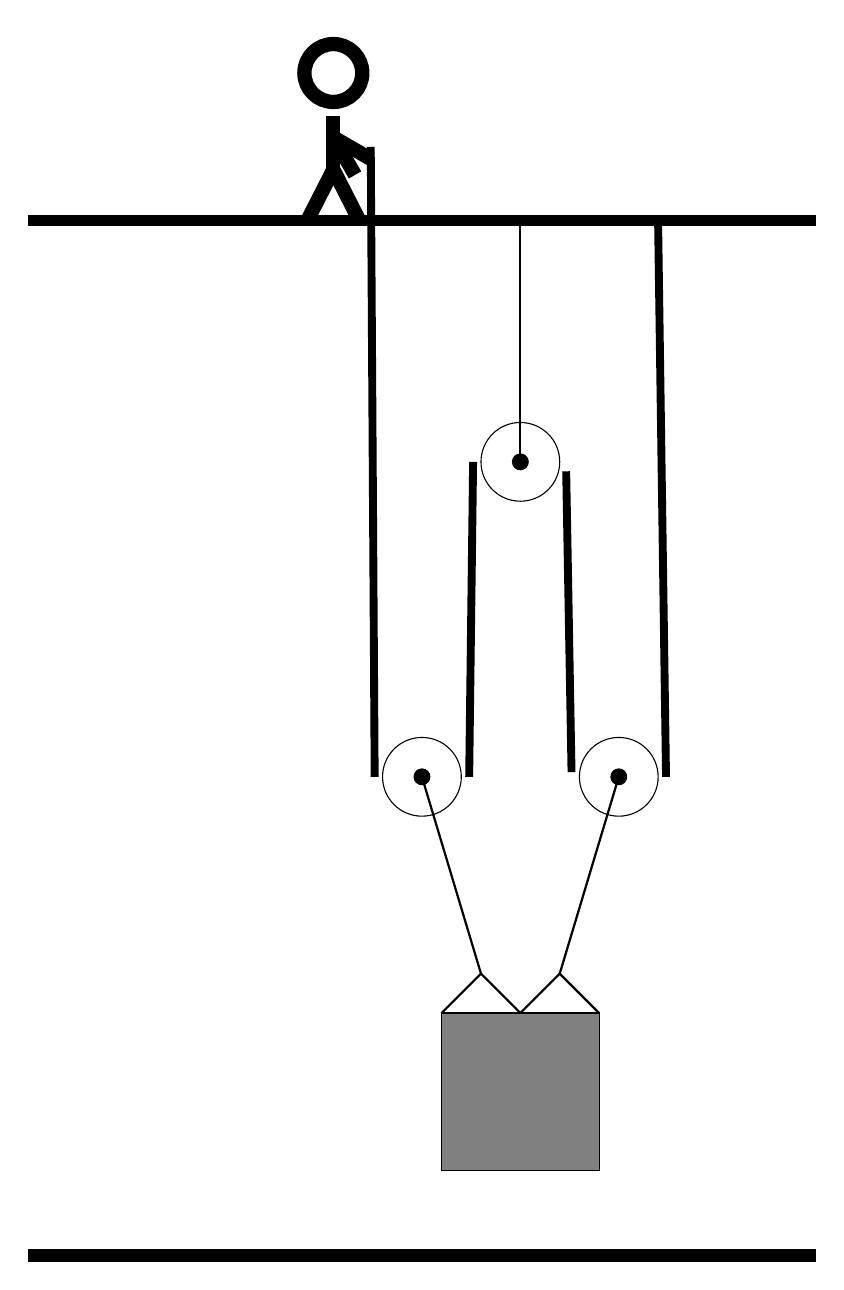
\begin{tikzpicture}
		%%%%% START %%%%%
		\draw[fill=black] (-4, 10) rectangle (6, 10.125);
		
		\draw (1, 3.0) circle (0.5);
		\draw[fill=black] (1, 3.0) circle (0.1);
		
		\draw (2.25, 7.0) circle (0.5);
		\draw[fill=black] (2.25, 7.0) circle (0.1);
		\draw[thick] (2.25, 7.0) -- (2.25, 10);
		
		\draw (3.5, 3.0) circle (0.5);
		\draw[fill=black] (3.5, 3.0) circle (0.1);
		
		\draw[thick] (3.5, 3.0) -- (2.75, 0.5);
		\draw[thick] (1, 3.0) -- (1.75, 0.5);
		\draw[thick]  (1.25, 0) -- (1.75, 0.5) -- (2.25, 0);
		\draw[thick]  (2.25, 0) -- (2.75, 0.5) -- (3.25, 0);
		\draw[fill=black!50] (1.25, 0) rectangle (3.25, -2);
		
		\draw[line width=1mm] (0.35, 11) --  (0.4, 3.0);
		\centerarc[line width=1mm](1, 3.0)(180:360:0.6);
		\draw[line width=1mm] (1.6, 3.0) -- (1.65, 7.0);
		\centerarc[line width=1mm](2.25, 7.0)(-20:180:0.6);
		\draw[line width=1mm](2.832, 6.88) -- (2.9, 3.06);
		\centerarc[line width=1mm](3.5, 3.0)(160:360:0.6);
		\draw[line width=1mm](4.1, 3.0) -- (4.0, 10);
		
		\node at (-0.07, 11.2) {\Strichmaxerl[10][120][-30]};
		
		\draw[fill=black] (-4, -3) rectangle (6, -3.15);
		%%%%% END %%%%%
	\end{tikzpicture}
\end{document}